\chapter{Kvantemekanikk}

Tidlig i fysikkundervisningen lærer vi at ved å se på summen av krefter på som virker på et objekt kan vi finne ut hvordan det vil bevege seg, $\sum\vec{F} = m\vec{a}$. Hvis vi prøver å bruke denne ligningen til å forutse hvordan et elektron beveger seg vil vi ofte\footnote{Det finnes tilfeller der Newtons lover gir en god beskrivelse av bevegelsen til elektroner, men i det generelle tilfellet er det ikke slik.} få feil resultat. Det viser seg at bevegelsen til elektroner---og andre tilstrekkelig små partikler og systemer av partikler---må beskrives på en helt annen måte. Det er det kvantemekanikken dreier seg om. Denne teksten vil ikke forsøke å gi en fullstendig innføring i kvantemekanikk, men bare diskutere litt generelle aspekter ved kvantemekanikken og gi en litt grundigere diskusjon av de elementene som er nødvendig for å forstå hvordan kvantedatamaskiner virker.

\section{Dobbelspalteeksperimentet}
Vi begynner med et kjent eksperiment som svært tydelig viser forskjellen mellom kvantemekanikk og klassisk mekanikk: dobbeltspalteeksperimentet. Før vi introduserer kvantemekanikken, la oss se på en klassisk versjon av eksperimentet. Figur \ref{fig:kvante:klassiskspalte} viser en skisse over oppsettet. Helt til venstre har vi en liten "kanon" som skyter ut små kuler i tilfeldige retninger. Helt til høyre har vi en plate som er i stand til å føle hvor den blir truffet. Midt mellom kanonen og detektorplaten er det en skjerm med to huller som er relativt små, men store nok til at kulene kan passere gjennom. For å forenkle diskusjonen skal vi betrakte systemet som om det kun har de to dimensjonene som er vist på figuren. Å ta med den tredje dimensjonen som finnes i den virkelige verden forandrer verken prinsippet i diskusjonen eller det essensielle i konklusjonen, så å ta med den ville bare vært en unødvendig komplikasjon.

Siden kulene blir skutt ut i tilfeldige retninger vil de fleste ikke treffe noen av hullene. Vi skal derimot kun bry oss om de som faktisk treffer et av hullene. En kule som treffer et hull kan enten gå rett gjennom hullet og fortsette rett frem i den retningen det hadde, eller den kan treffe kanten av hullet å få endret retningen sin litt eller mye. I figur \ref{fig:kvante:klassisktreff} er det skissert hvordan treffpunktene på detektorplaten fordeler seg. Skissen lengst til venstre viser fordelingen av kun de kulene som gikk gjennom det øvre hullet\footnote{Vi bør egentlig tenke oss at systemet ligger flatt slik at ikke tyngdekraften påvirker fordelingen, men siden det på figuren er et øvre og et nedre hull er det enklest å omtale de på denne måten.}. Skissen i midten viser fordelingen av kun de kulene som gikk gjennom det nederste hullet. Skissen lengst til høyre viser fordelingen av alle treffpunktene. Den siste fordelingen er naturlig nok lik summen av de to første. Dette betyr at hvis vi ønsker å finne sannsynligheten for at et bestemt punkt på detektorplaten blir truffet kan vi enkelt regne det ut som
\begin{displaymath}
	p(x) = p_1(x) + p_2(x).
\end{displaymath}
Her viser koordinaten $x$ til hvilket punkt på detektorplaten vi vil undersøke. Vi kan for eksempel la $x=0$ være punktet som ligger rett bak midt mellom hullene, og la $x$ måle hvor høyt over eller lavt under dette punktet er. $p_1(x)$ svarer til sannsynligheten for at en kule går gjennom det øvre hullet og så treffer punktet $x$. Tilsvarende er $p_2(x)$ sannsynligheten for at en kule går gjennom det nedre hullet og treffer punktet $x$. 
\begin{figure}[tp]
	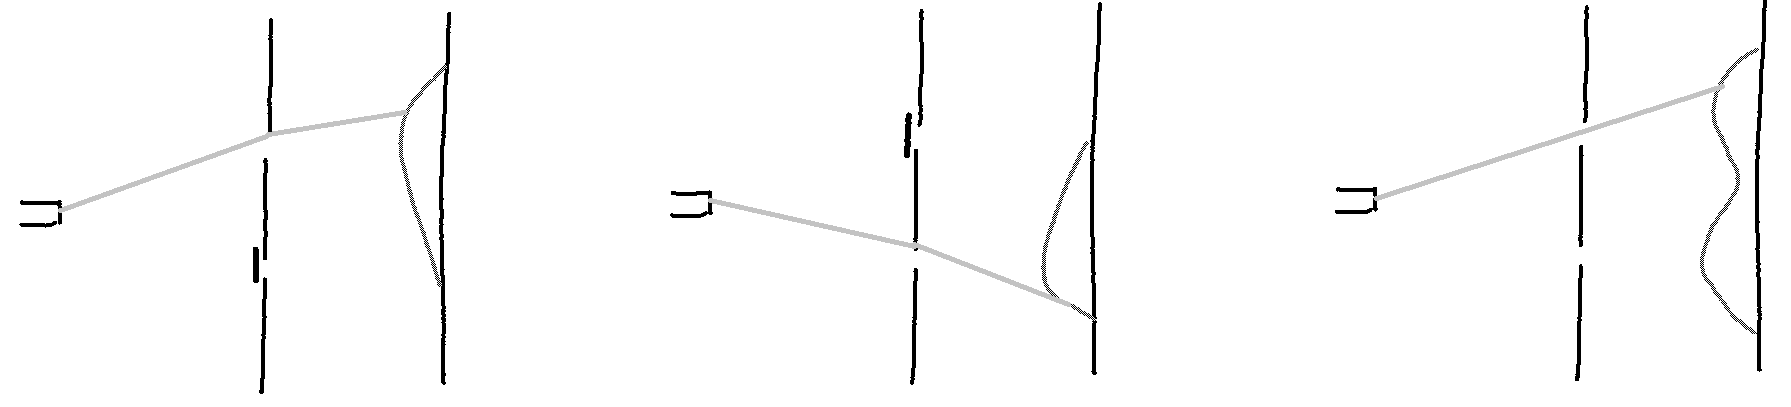
\includegraphics[width=\textwidth]{./dobbeltspalte1}
	\caption{Skisse av dobbeltspalte-eksperimentet utført med klassiske kuler. De grå linjene indikerer eksempler på baner kulene tar fra kilden til detektorskjermen. Kurven som er skissert på skjermen viser fordelingen av treffpunkter. Skissen til venstre og i midten viser fordelingen av treff dersom et av hullene er blokkert. Skissen til høyre viser fordelingen av treff dersom begge huller er åpne. Merk at treffordelingen med begge huller åpne ganske enkelt er summen av treffordelingene der et av hullene er blokkert.}
	\label{fig:kvante:klassisktreff}
\end{figure}

Vi bytter nå ut kanonen vår med en "elektronkanon"---en kilde som skyter ut elektroner i tilfeldige retninger. Oppsettet for øvrig er likt---selvfølgelig med den tilpasning at vi nå velger en skjerm med huller som er mye mindre siden elektronene er mye mindre enn kulene, og en annen type detektorskjerm siden det er elektroner som skal detekteres nå. Fremdeles skal hullene være store nok til at elektronene kan gå gjennom, men små nok til at det er en vesentlig sannsynligehet for at de vil treffe kanten av hullet og endre retning. Naivt sett skulle man forvente at vi får se akkurat det samme som i tilfellet med kuler, men det er absolutt ikke det som skjer.

Med kun ett hull åpent skjer ikke den store endringen, men å ha begge hullene åpne endrer alt. Dette er illustrert i figur \ref{fig:kvante:kvantetreff}. Hvis vi insisterer på å tolke elektronene som kuler som beveger seg fra kilden, gjennom et av hullene og til detektorskjermen gir ikke denne treffordelingen noen mening. Hvis vi dermed tolker elektronene som bølger er fordelingen akkurat slik man skulle forventet, se figur \ref{fig:kvante:interferens}. Bølgen brer seg utover fra kilden, og de delene av bølgefronten som treffer et hull fortsetter på andre siden av skjermen. Hullene blir da essensielt sett nye kilder til bølger som brer seg utover. Når bølgene fra de to hullene treffer hverandre vil resultatet bli en sum av de to bølgene: Hvis to bølgetopper treffer hverandre blir resultatet dobbelt så stort som den enkelte bølgen i seg selv. Hvis en bølgetopp treffer en bølgebunn blir det ikke noe utslag i det hele tatt. Dette forklarer hvorfor treffordelingen på detektorskjermen viser en stor topp i midten, og også noen områder uten treff i det hele tatt.

\begin{figure}[tp]
	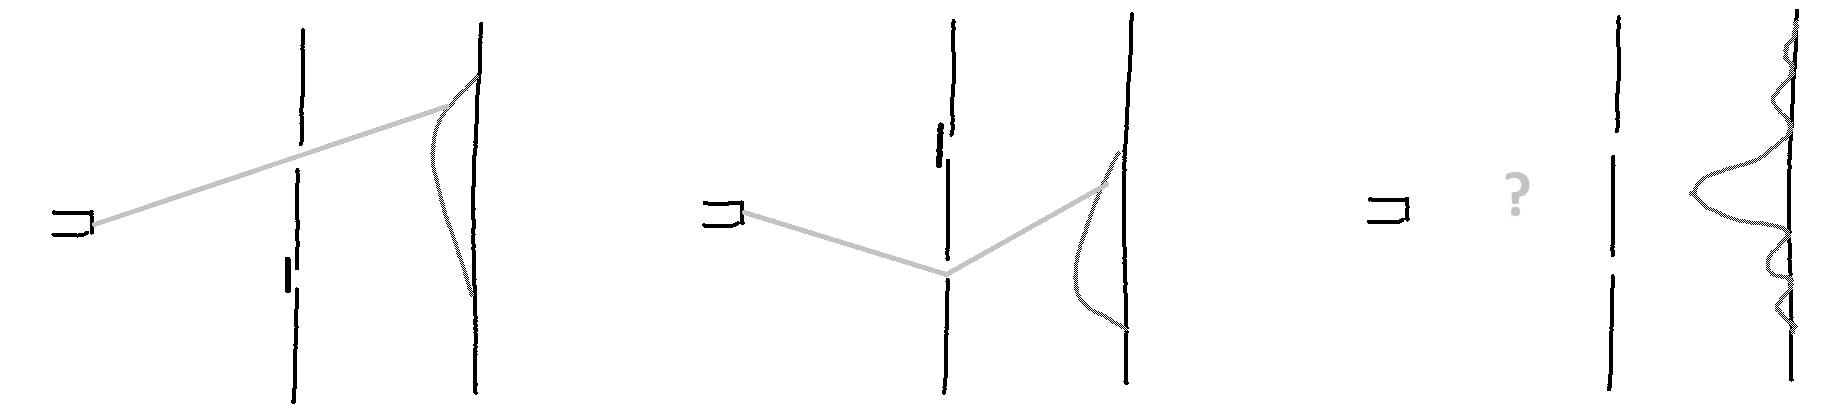
\includegraphics[width=\textwidth]{./dobbeltspalte2}
	\caption{Skisse av dobbeltspalte-eksperimentet utført med elektroner. De grå linjene indikerer eksempler på baner elektronene tar fra kilden til detektorskjermen. Kurven som er skissert på skjermen viser fordelingen av treffpunkter. Merk at fordelingen når et av hullene er blokkert ser likt ut som i det klassiske tilfellet, men når begge hullene er åpne blir fordelingen helt annerledes.}
	\label{fig:kvante:kvantetreff}
\end{figure}

Denne bølgetolkningen av elektronet er imidlertid ikke hele historien. Hvis vi nå gjør eksperimentet og sørger for at kun ett elektron passerer gjennom apparatet til enhver tid får vi fremdeles treffordelingen som er indikert i figur \ref{fig:kvante:kvantetreff}. Men hvert enkelt elektron treffer ikke litt her og litt der på detektorskjermen slik en bølge ville gjort. Hvert elektron treffer detektorskjermen på et veldefinert sted. Forklaringen på hvorfor treffordelingen blir som den blir må altså inneholde både denne bølgelike bevegelsen gjennom systemet, og den partikkel-like måten å treffe detektorskjermen. 

\section{Bølgefunksjonen $\psi$}
\label{sec:kvante:psi}
En kvantemekanisk beskrivelse av verden viser seg å være svært annerledes enn det vi er vant med. Det viser seg at hvis du vil forsøke å forutsi hvilket resultat en måling---for eksempel av posisjonen eller farten til et elektron---vil gi må du nøye deg med å forutsi hvordan sannsynligheten for ulike måleresultater du kan få er. Dette dreier seg ikke om den vanlige måleusikkerheten som skyldes at måleinstrumentet ikke er perfekt, men det er en underliggende fysisk realitet. La oss for konkrethet se på posisjonen til et elektron. I klassisk fysikk som vi kjenner den fra før ville vi benevnt posisjonen med en vektor
\begin{displaymath}
	\vec{r} = (x,y,z)
\end{displaymath}
som beskriver posisjonen til elektronet med tre koordinater som i prinsippet kan bestemmes eksakt. Hvis vi kjenner alle kreftene som virker kan vi beregne hvordan posisjonen varierer med tiden,
\begin{displaymath}
	x = x(t),\quad y = y(t),\quad z=z(t),
\end{displaymath}
slik at vi vet nøyaktig hvor elektronet er også på et vilkårlig tidspunkt i fremtiden.

En kvantemekanisk beskrivelse av elektronet innebærer en såkalt bølge\-funksjon som forteller oss om sannsynligheten for å finne elektronet på et bestemt sted. I det videre vil jeg begrense meg til å beskrive endimensjonal bevegelse for å forenkle notasjonen, men konseptet kan enkelt utvides til tre dimensjoner. Til å beskrive elektronets posisjon bruker vi funksjonen $\psi(x)$, men denne må tolkes på en helt annen måte enn vektoren $\vec{r}$ ovenfor. For det første vil $\psi(x)$ normalt ha en verdi som er ulik null i mer enn ett punkt, noe som betyr at elektronet ikke har en fast definert posisjon, men kan tenkes å være flere steder. Merk at dette faktisk ikke er et uttrykk for at det finnes informasjon om hvor elektronet egentlig er som vi mangler, men at posisjonen til elektronet ikke er fast definert\footnote{Denne bemerkningen fortjener egentlig en lang diskusjon, men dette er ikke stedet for denne diskusjonen. Det er skrevet mye om dette andre steder.}. Figur \ref{fig:kvante:psix} viser to mulige funksjoner $\psi(x)$ som beskriver posisjonen til et elektron som befinner seg ved eller nær $x=1~\mathrm{m}$. Den stiplete blå linjen er kun ulik null i et relativt lite område nær $x=1~\mathrm{m}$. Dette betyr at vi har en ganske stor visshet om hvor elektronet som beskrives av denne $\psi$-funskjonen er. Den heltrukne røde linjen er mer fordelt utover og innebærer derfor at det er et større område der det er sannsynlig at vi vil finne elektronet. 
\begin{figure}[htp]
\begin{center}
	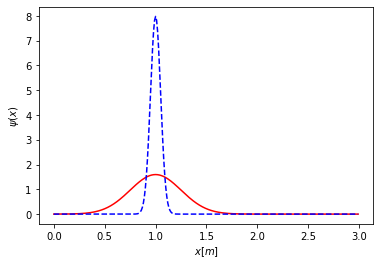
\includegraphics[width=.5\textwidth]{./psix}
	\caption{}
	\label{fig:kvante:psix}
	\end{center}
\end{figure}

Hva skjer så når vi prøver å måle hvor elektronet er? Da vil vi---uansett hvor konsentrert eller utspredt bølgefunksjonen som beskriver det er---finne elektronet lokalisert i ett punkt\footnote{Selvfølgelig med en presisjon som er begrenset av måleinstrumentet vi bruker.}. Dette innebærer at når vi måler hvor elektronet er endrer vi samtidig bølgefunksjonen som beskriver elektronet til å bli mye mer konsentrert rundt ett punkt, men dette punktet trenger ikke nødvendigvis å være der den tidligere hadde maksimum. Det vil imidlertid alltid være et sted der $\psi(x)$ før målingen var ulik null. Hvis vi kjenner bølgefunksjonen før vi måler kan vi bruke den til å beregne sannsynligheten for å finne elektronet i ulike områder. Det gjør vi ved å integrere over kvadratet av absoluttverdien av $\psi(x)$. For eksemel er sannsynligheten for å finne elektronet et sted mellom $x=0,75~\mathrm{m}$ og $x=0,76~\mathrm{m}$
\begin{equation}
	P ( 0,75~\mathrm{m}<x<0,76~\mathrm{m}) = \int_{0,75~\mathrm{m}}^{0,76~\mathrm{m}}|\psi(x)|^2\d x
	\label{eq:kvante:prob}
\end{equation}
Noen bemerkninger om funksjonen $\psi(x)$
\begin{enumerate}
\item
For at integralet i ligning (\ref{eq:kvante:prob}) skal gi en meningsfull sannsynlighet må funksjonen $\psi(x)$ oppfylle et normaliseringskrav, nemlig 
\begin{displaymath}
	1 = \int_{-\infty}^\infty |\psi(x)|^2\d x.
\end{displaymath}
Dette betyr for det første at sannsynligheten for å finne elektronet et eller annet sted er 1. For det andre, siden $|\psi(x)|^2 \geq 0$ overalt vil vi da være sikret å finne sannsynlighet $P\leq1$ dersom vi integrerer over et kortere intervall.
\item
Når vi integrerer over kvadratet av absoluttverdien til funksjonen ($|\psi|^2$) og ikke bare over kvadratet av funksjonen ($\psi^2$) er det fordi det viser seg at vi generelt må tillate $\psi(x)$ å ha komplekse verdier. I enkelte sammenhenger er dette av stor betydning, men i denne teksten får vi ikke behov for å studere dette videre.
\item
Vi har så langt diskutert bølgefunksjonen som en helt vanlig funksjon som tar inn ett tall (posisjonen) og gir ut ett tall (som riktignok kan være komplekst) som kan relateres til sannynligheten for å finne elektronet akkurat der. Generelt vil vi trenge litt mer kompliserte konstruksjoner. En første enkel utvidelse av dette er å ta med de to andre romlige koordinatene samt å ta med en tidsavhengighet som beskriver at bølgefunksjonen endrer seg når tiden går\footnote{En vanlig konvensjon er å bruke stor $\Psi$ for å betegne en bølgefunksjon som avhenger av både rom- og tidskoordinater, mens man bruker liten $\psi$ dersom bølgefunksjonen kun avhenger av de romlige koordinatene, men ikke endrer seg når tiden går.}:
\begin{displaymath}
	\Psi(x,y,z,t).
\end{displaymath}
Videre er det i en del sammenhenger---blant annet en vi skal se på snart og få mye bruk for i resten av denne teksten---ofte nyttig å la bølgefunksjonen gi ut en vektor i stedet for bare et tall:
\begin{displaymath}
	\Psi(x,y,z,t) = \left[ \begin{array}{cc}\phi_1(x,y,z,t) \\ \phi_2(x,y,z,t) \end{array}\right],
\end{displaymath}
der $\phi_1(x,y,z,t)$ og $\phi_2(x,y,z,t)$ er vanlige funksjoner som gir ut (muligens komplekse) tall.
\end{enumerate}

\section{Schr{\"o}dingerligningen}
Gitt en bølgefunksjon $\Psi(x,y,z,t)$ og en funksjon $V(x,y,z)$ som beskriver den potensielle energien som funksjon av posisjonen kan vi finne tidsutviklingen til bølgefunksjonen ved å løse en partiell differensialligning som er kjent som Schr{\"o}dingerligningen (her skrevet opp med bare \'en romlig koordinat):
\begin{displaymath}
	i\hbar\frac{\partial}{\partial t}\Psi(x,t) = \left[ - \frac{\hbar^2}{2m}\frac{\partial^2}{\partial x^2} + V(x)\right]\Psi(x,t)
\end{displaymath}
Her er $m$ massen til partikkelen som beskrives, i vårt tilfelle elektronmassen, og $\hbar = \frac{h}{2\pi} = 1,055\times10^{-34}~\mathrm{Js}$ er den reduserte Planck-konstanten. Schr{\"o}dingerligningen spiller omtrent samme rolle i kvantemekanikken som Newtons andre lov ($\Sigma \vec{F} = m\vec{a}$) spiller i klassisk mekanikk: Den tillater oss å beregne hva som vil skje i fremtiden med kunnskap om hvordan tilstanden er nå. Det er imidlertid noen vesentlige forskjeller. For det første er det bare presisjonen i målingene som begrenser presisjonen i forutsigelsen i klassisk mekanikk. I kvantemekanikk kan vi---som allerede diskutert---kun beregne sannsynligheten for ulike måleresultater, ikke forutsi med sikkerhet hva vi vil måle. Så selv om vi skulle kjenne bølgefunksjonen slik den er nå uten usikkerhet, og dermed kunne forutsi hvordan den vil være i fremtiden uten usikkerhet vil vi fremdeles ikke vite hvilket måleresultat vi ender opp med. For det andre kan Newtons andre lov brukes ``baklengs'': Hvis vi måler hva posisjon og fart er nå kan vi bruke det til å regne ut hva posisjon og fart var på et tidligere tidspunkt. Siden en måling påvirker bølgefunksjonen kan vi ikke bruke Schr{\"o}dingerligningen til å finne ut hvordan bølgefunksjonen var på et tidspunkt før vi målte f.eks. posisjonen til elektronet.

I en generell innføring til kvantemekanikk legges det som regel stor vekt på å løse Schr{\"o}dingerligningen for ulike potensialer $V(x)$. Dette er ikke nødvendig for diskusjonen videre i denne teksten, så det problemet vil ikke bli diskutert videre her.

\section{Spinn}
\label{sec:kvante:spinn}
En del subatomære partikler, inkludert elektronet som vi fokuserer mest på her, har en egenskap som heter spinn. Ordet spinn antyder at det er noe som snurrer rundt, men det er ikke tilfellet. Det er snakk om en iboende egenskap i partikkelen. Likevel kan rotasjonen til en snurrebass være en brukbare analogi for \emph{enkelte aspekter} ved spinnet. Spinn er en vektor som altså har både en størrelse og en retning. I snurrebassanalogien svarer størrelsen til hvor fort den roterer, mens retningen svarer til retningen rotasjonsaksen peker. Positiv retning defineres slik at snurrebassen roterer mot klokken når vi ser den fra den positive siden. Det viser seg at spinnet til subatomære partikler alltid er på formen $\frac{a}{2}\hbar$ der verdien av $a$ avhenger av hvilken partikkel det dreier seg om. Partikler der $a$ er et partall slik at spinnet er et heltall multiplisert med $\hbar$ kalles bosoner. Partikler der $a$ er et oddetall kalles fermioner. Elektronet har $a = 1$ slik at spinnet til elektronet har størrelse $\half\hbar$. Ofte skriver vi dette bare som spinn \half, og jeg vil bruke denne konvensjonen i det videre.

I det videre bryter analogien med en snurrebass fullstendig sammen. I stedet for å måle hvilken retning spinnet til et elektron peker er det enklere å måle projeksjonen av spinnet inn på en vilkårlig akse. Hvis vi gjør dette med en snurrebass vil vi finne en verdi av projeksjonen $s$ slik at  $-S < s < +S$, der $S$ er størrelsen til spinnet. $s=+S$ og $s=-S$ svarer til at aksen vi måler langs er enten parallell eller antiparallell med rotasjonsaksen. $s=0$ svarer til at aksen vi måler langs står normalt på rotasjonsaksen. Når vi gjør denne målingen på et elektron finner vi alltid $+\half$ eller $-\half$ uansett hvilken akse vi måler langs. Sett nå at vi preparerer et elektron med spinnet sitt rettet langs den positive $x$-aksen. Hvis vi nå velger å måle projeksjonen av spinnet på $x$-aksen vil vi med sikkerhet ende opp med resultatet $+\half$. Hvis vi derimot velger å måle projeksjonen av spinnet langs positiv $z$-akse (som står normalt på $x$-aksen) vil vi ende opp med å måle enten $+\half$ eller $-\half$ med 50\% sannsynlighet for hver av verdiene. Hvis vi etter å ha målt projeksjonen langs $z$-aksen igjen måler projeksjonen langs $x$-aksen vil vi ikke lenger med sikkerhet måle $+\half$. Derimot vil vi nå bare ha 50\% sannsynlighet for at målingen viser $+\half$, mens det også er 50\% sannsynlighet for å få verdien $-\half$. 

Som en avslutning av denne første diskusjonen av spinntet tar jeg med at hvis vi igjen preparerer elektronet med spinn opplinjert med $x$-aksen og deretter måler projeksjonen av spinnet på en akse som danner en vinkel $\theta$ med $x$-aksen da blir sannsynlighetene for de to mulige resultatene av målingen
\begin{displaymath}
	P\left(+\half\right) = \cos^2\theta, \quad P\left(-\half\right) = 1- \cos^2\theta = \sin^2\theta.
\end{displaymath}

\section{Måleproblemet}
Både i diskusjonen av posisjonen til elektronet i avsnitt \ref{sec:kvante:psi} og retningen til elektronspinnet i avsnitt \ref{sec:kvante:spinn} var det en underliggende observasjon som ikke ble tydelig formulert:
\begin{quote}
Når vi utfører en måling på et kvantemekanisk system kan vi ikke unngå å samtidig påvirke systemet.
\end{quote}
Dette er helt sentralt, og viser en tydelig forskjell på klassisk mekanikk og kvantemekanikk. I klassisk mekanikk ser vi på objekter som er store nok til at vi kan måle størrelser som for eksempel posisjon eller fart uten relevant påvirkning av størrelsen vi ønsker å måle. Vi kan for eksempel måle posisjonen til en ball ved å \emph{se på den} mens vi har en linjal like ved for å definere måleskalaen. For at vi skal kunne se ballen må det skinne lys på den som reflektres inn i øynene våret. Lyset består av små partikler som kalles fotoner som treffer overflaten til ballen før de sendes videre til, blant annet, øynene våre. Når fotonene treffer ballen gir de den en liten dytt, så i prinsippet kan de endre posisjonen til ballen i prosessen. I praksis er imidlertid bevegelsesmengden til fotonene så liten at de ikke gir noen relevant kraftvirkning på ballen. Derfor kan vi jobbe som om måleprosessen ikke i det hele tatt påvirker det vi ønsker å måle. Dette er ikke tilfellet når vi kommer til kvantemekanikk.

Vi fortsetter å bruke elektronet som eksempel. Massen til et elektron er $m_e = 9,1\times10^{-31}~\mathrm{kg}$. Bevegelsesmengden til et foton avhenger av bølgelengden. Om vi ser på et foton omtrent midt i det synlige spekteret ($\lambda = 550~\mathrm{nm}$) har det bevegelsesmengden $p = \frac{h}{\lambda} = 1,2\times10^{-27}~\mathrm{kg\, m/s}$. Hvis vi bruker dette fotonet til å måle hvor elektronet er vil vi altså samtidig gi elektronet en så kraftig dytt at det etterpå vil ha stor fart bort fra det stedet det var. Slik er det med alle målinger i kvantemekanikken---måleprosessen påvirker systemet vi måler på. Og enda verre, jo mer nøyaktig vi prøver å måle, jo mer vil vi ende opp med å påvirke systemet. Generelt kan vi si at hvis vi ikke kan gjøre målingen på en slik måte at påvirkningen på systemet er neglisjerbar så må vi behandle systemet som kvantemekanisk. Hvis vi derimot kan måle på det uten at målingen gir noen relevant påvirkning på systemet kan vi behandle det med vanlig klassisk mekanikk. 

Det finnes noen spesialtilfeller der vi tilsynelatende unslipper dette måle\-problemet, selv når vi jobber med et system som må behandles kvante\-mekanisk. Et viktig eksempel, og det eneste jeg vil se på her, er gjentatte målinger av elektronspinnet. I avsnitt \ref{sec:kvante:spinn} diskuterte jeg hvordan projeksjonen av spinnet på en akse antar tilfeldige verdier. Men hvis vi repeterer gjentatte målinger langs den samme aksen får vi hele tiden samme resultat. Med andre ord, hvis spinnet er opplinjert med $x$-aksen og vi fortsetter å måle projeksjonen av spinnet inn på $x$-aksen vil ikke målingen endre spinnet. Hvis vi derimot velger å måle spinnet langs en annen akse, for eksempel $z$-aksen, vil målingen påvirke spinnet som diskutert ovenfor.

\section{Sammenfiltring}
Så langt har diskusjonen gitt inntrykk av at hvert enkelt elektron---og andre objekter også for den saks skyld---har hver sin bølgefunksjon. Dette er ikke realiteten. I prinsippet må hele universet beskrives av en felles bølgefunksjon som beskriver alt som er i det. Heldigvis kan vi i mange tilfeller bruke en enklere beskrivelse og likevel få en god representasjon av virkeligheten. Situasjonen er ganske lik til klassisk fysikk: Når vi beregner banen til en stein som blir kastet tar vi hensyn til tyngdekraften fra jorden, men ikke tyngdekraften fra solen, månen og de andre planetene i solsystemet. I prinsippet skulle tyngdekraften fra alt annet i universet vært med i beregningen, men tyngdekraften fra jorden er så mye større enn de andre bidragene at vi kun trenger å ta hensyn til denne. Tilsvarende argument tillater oss i mange tilfeller å regne med \'en bølgefunksjon per objekt i kvantemekanikken. Men det finnes også tilfeller der to eller flere objekter må beskrives av en felles bølgefunksjon for å få en riktig beskrivelse. Når dette er tilfellet sier vi at objektene er \emph{sammenfiltret}. 

Som eksempel på sammenfiltring skal vi se på spinnet til to elektroner. Det er mulig å preparere paret av elektroner slik at summen av spinnet deres målt langs en akse er null. Siden hvert av elektronene kun har muligheten $+\half$ og $-\half$ må altså spinnet til de to elektronene peke hver sin vei. Det spesielle med en sammenfiltret tilstand er at det ikke er slik at det ene elektronet har spinn $+\half$ og det andre $-\half$. I hvert fall ikke før vi har målt. Begge elektronene er i en superposisjon mellom begge mulighetene, men straks vi måler spinnet til det ene elektronet vet vi også hva måleresultatet vil bli når vi måler spinnet til det andre. For å understreke hvor uvant dette er kan vi se på et konkret eksempel. Vi preparerer sammenfiltrede paret av elektroner og plasserer dem i hvert sitt laboratorium adskilt med $3000~\mathrm{km}$. Siden det ikke er mulig å sende noe signal raskere enn lyshastigheten vil det ta minst $10~\mathrm{ms}$ å sende et signal fra det ene laboratoriet til det andre. På et avtalt tidspunkt måler man spinnet til det ene elektronet, og $1~\mathrm{ms}$ senere måler man spinnet til det andre elektronet. Selv om elektronene er for langt fra hverandre til å kunne rekke å kommunisere finner man alltid perfekt korrelasjon: det ene har spinn $+\half$ og det andre har spinn $-\half$. 

En fristende forklaring på hvordan elektronene kan ha denne perfekte korrelasjonen uten tid til å kommunisere er at i realiteten hadde det ene elektronet hele tiden spinn $+\half$ og det andre hadde hele tiden spinn $-\half$. Det var bare det at vi ikke hadde nok informasjon til å vite hvilken som hadde hva frem til vi målte. I 1964 publiserte John Steward Bell en artikkel der han beskrev hvordan man kunne teste om dette faktisk var tilfellet~\cite{PhysicsPhysiqueFizika.1.195}. Jeg skal ikke forsøke å gi en fullstendig beskrivelse av testen her, men bare skissere eksperimentet Bell foreslo. I likhet med eksperimentet jeg har skissert ovenfor skal man også her gjentatte ganger måle spinnet til to sammenfiltrede elektroner som er separert slik at de ikke får tid til å sende et signal fra det ene til det andre. I eksempelet ovenfor målte vi alltid spinnet langs den samme aksen. I Bell sitt eksperiment skal vi måle spinnet langs \'en av tre retninger som er separert med $120^\circ$. Hvilken retning som brukes i hver enkelt måling velges tilfeldig i hvert av de to laboratoriene, og beslutningen gjøres så kort tid før målingen blir gjort at det ikke er tid for et lyssignal å gå fra det ene laboratoriet til det andre. Det viser seg da at korrelasjonen mellom måleresultatene fra de to laboratoriene vil bli ulik avhengig av om
\begin{enumerate}
\item
elektronene på forhånd har et fast definert spinn som vi ikke har nok informasjon til å vite (forutsigelsen til klassisk fysikk), eller
\item
elektronene er begge i en superposisjon mellom de to mulig utfallene av målingen helt frem til vi har målt spinnet til minst ett av elektronene (forutsigelsen til kvantemekanikk).
\end{enumerate}
Eksperimentet har blitt utført med mange forskjellige variasjoner\footnote{De fleste eksperimentene ser på polarisasjonen til fotoner i stedte for spinnet til elek\-troner fordi dette er teknisk enklere å jobbe med, men prinsippet er det samme.}, de første gangene av John Clauser og Stuart Freedman\cite{PhysRevLett.28.938} og Alain Aspect, Philippe Grangier og G\'erard Roger \cite{PhysRevLett.47.460}, og det er ikke mye tvil om at det er kvantemekanikken som forutsier resultatet riktig.